\section{Results}

\begin{minipage}{\linewidth}
    \centering
    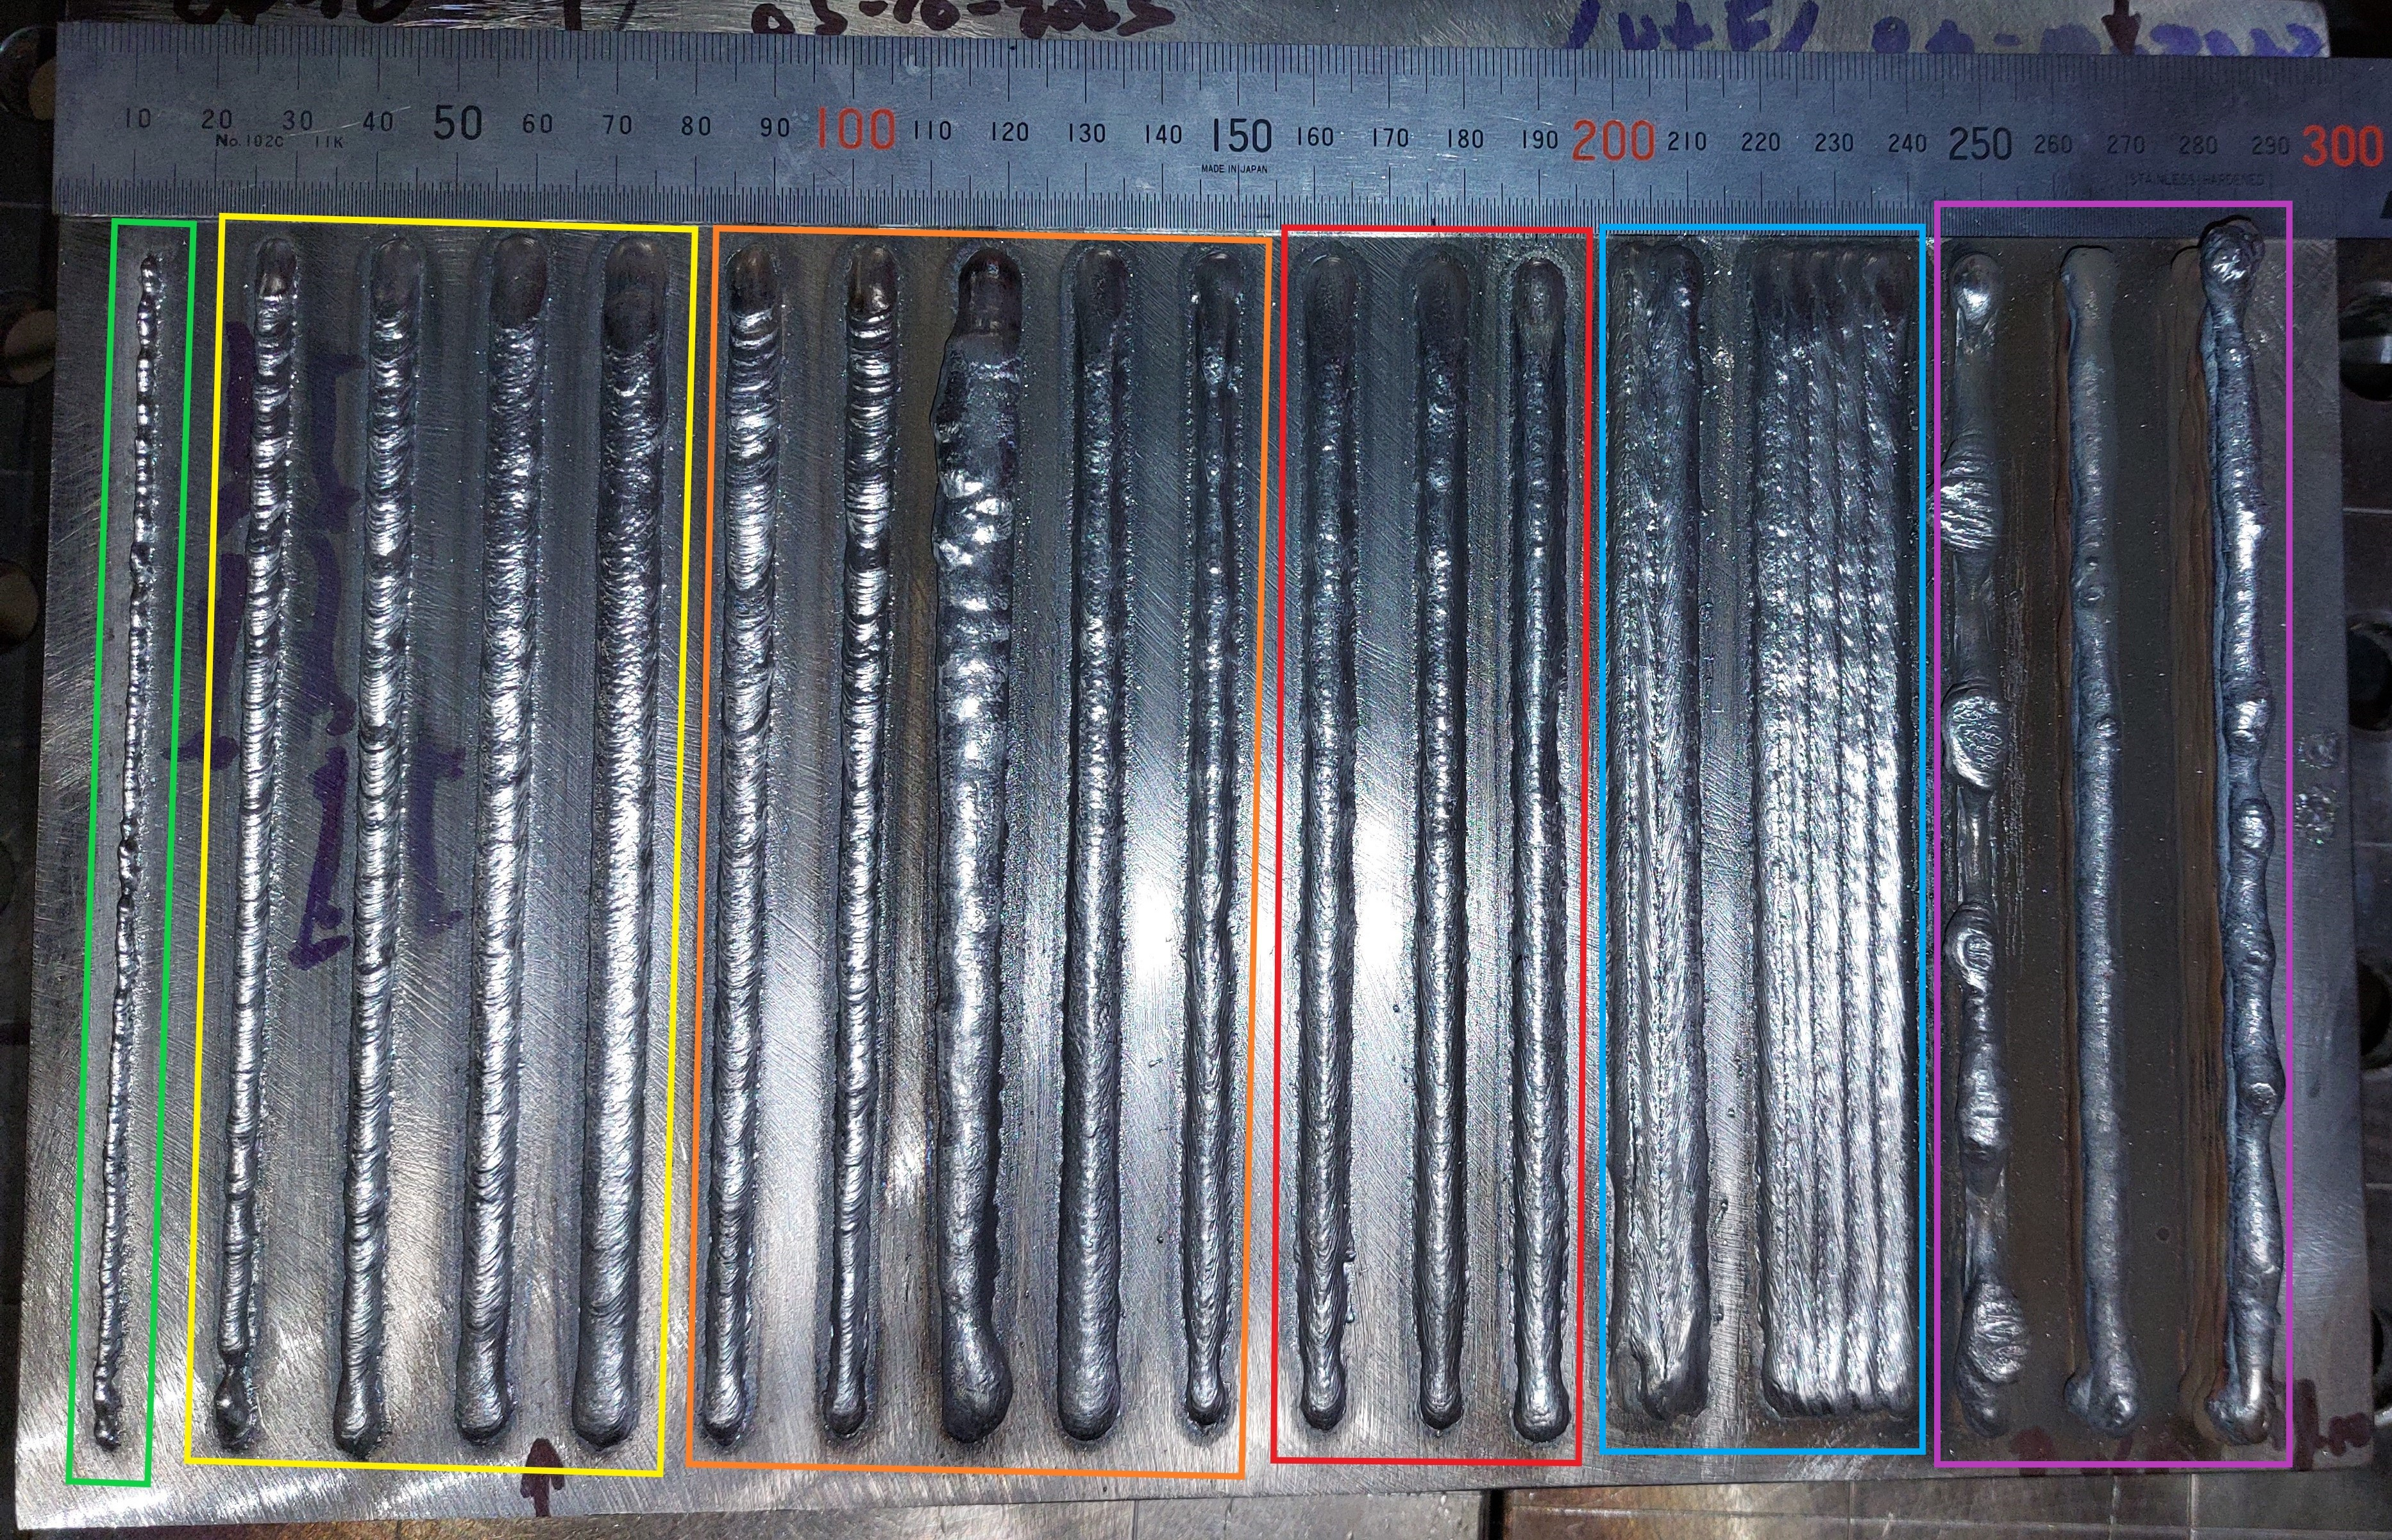
\includegraphics[width=\linewidth]{images/all_welds_boxes.jpg}
    \captionof{figure}{Initial welding tests}
    \label{fig:all_welds}
\end{minipage}

The results of the experiments correspond to the milestones set out in the Methods section. As shown in \autoref{fig:all_welds}, the initial welding tests were successful and have been marked with colored boxes to indicate the milestones they correspond to. The figure includes a ruler for scale. All exact travel speeds and feed rates are listed in the Appendix XXX.

\textbf{Green box}: Minimum weldability for single beads. A travel speed of 0.3 m/min and feed rate ramp from 2-1.4 m/min was used. The weld was thin but unbroken, thus showing the minimum weldability and wettability of the material on this baseplate.

\textbf{Yellow box}: Minimum weld quality for single beads. These tests were all conducted at 0.3 m/min travel speed, and were feed rate ramps from 3.8-13.6 m/min to test the entire available range. 8.5 m/min (bead 4) was found to be an acceptable condition for single bead welds.

\begin{figure}[H]
    \centering
    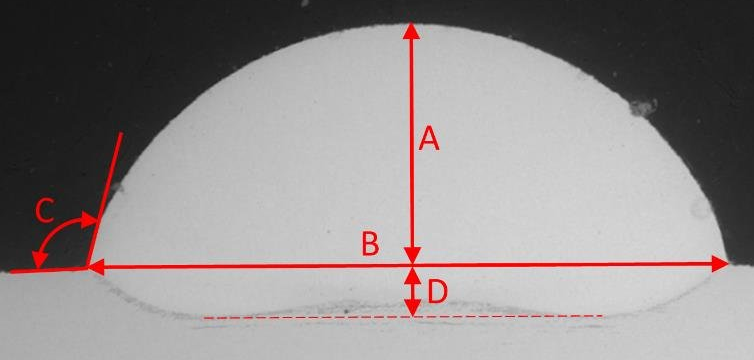
\includegraphics[width=\linewidth]{images/bead_geometry.png}
    \caption{Bead geometry \cite{Dinovitzer_Chen_Laliberte_Huang_Frei_2019}}
    \label{fig:bead_geometry}
\end{figure}

\textbf{Orange box}: Minimum weld quality for overlapping beads.
The bead wall angle, shown as angle $c$ in \autoref{fig:bead_geometry}, should be above 90 $\deg$ for overlapping beads to mix well with each other. All previous beads were quite "steep" ($c \approx 90 \deg$), and in order to get the beads to spread better, higher energy inputs are required. These next tests all used travel speed ramps with fixed feed rates.

Beads 6-8 used 8.5 m/min feed rate and 0.5-0.2 m/min travel rate with varying arc length corrections to try and create higher voltages, although an overprinting error ocurred with bead 8. In an attempt to increase spreading even further, beads 9-10 used 14.5 m/min feed rate and tested the 0.4-1.3 m/min travel speed range, finding 0.8 to be an acceptable condition for overlapping beads.

\textbf{Red box}: Process stability of overlapping beads.
In the red box, this condition was tested with small variations to the initial weld conditions due to the apparent necking ocurring at the start of the bead. SFI time was increased from 0.1 seconds to 1 second to stabilize material deposition, and the initial current was increased to 125\% of the main current.
This did indeed improve the necking somewhat, but induced too much deposition at the weld start. The bead width of the stable overlap condition (0.8 m/min travel speed, 14.5 m/min feed rate) was 5.5 mm.

\textbf{Blue box}: Minimum weld quality of overlapping beads.
The resulting overlap condition from the previous tests was tested with 3-bead overlap with 60\% of the bead width separation, and 5-bead overlap with 70\% separation. The 3-bead overlap showed too much accumulation of material between beads, which is why the distance was slightly increased, resulting in a relatively smooth surface for pieces requiring wider layers.

\textbf{Purple box}: Process stability over many single-bead layers. The three beads shown here are attempts at building walls, all with an average layer height of 2 mm. All three attempts resulted in the same deposition inconsistencies and significant loss of process stability.
For all walls, an interpass temperature of 50$\deg$ was used to ensure that no defects due to overheating might occur. These thermal measurements were sometimes not indicative of the temperature at the topmost layer (due to thermocouple placement or MaxQ thermal camera calibration issues).
The first wall got there after 3 layers, the second after 6, and the heat input was lowered by around 30\% by reuducing the feed rate from 8.5 m/min to 7.3. This allowed the third wall to stay stable up to 10 layers, but the deposition inconsistencies were still present.

Several possibilities for the defects were considered: the arc length may have been too large and not constant enough, allowing the arc to wander and the melt pool to deposit inconsistently. Weld cavities in previous layers would thus be amplified in subsequent layers, and this would be the reason for regularly occuring defects after a set number of layers. The process stability would also be aggravated by a higher heat input.

A final wall was printed on a separate baseplate with a lower heat input at 5.5 m/min feed rate as opposed to 7.3. Defects still ocurred after around 10 layers, as shown in \autoref{fig:big_wall_1}.

\begin{minipage}{\linewidth}
    \centering
    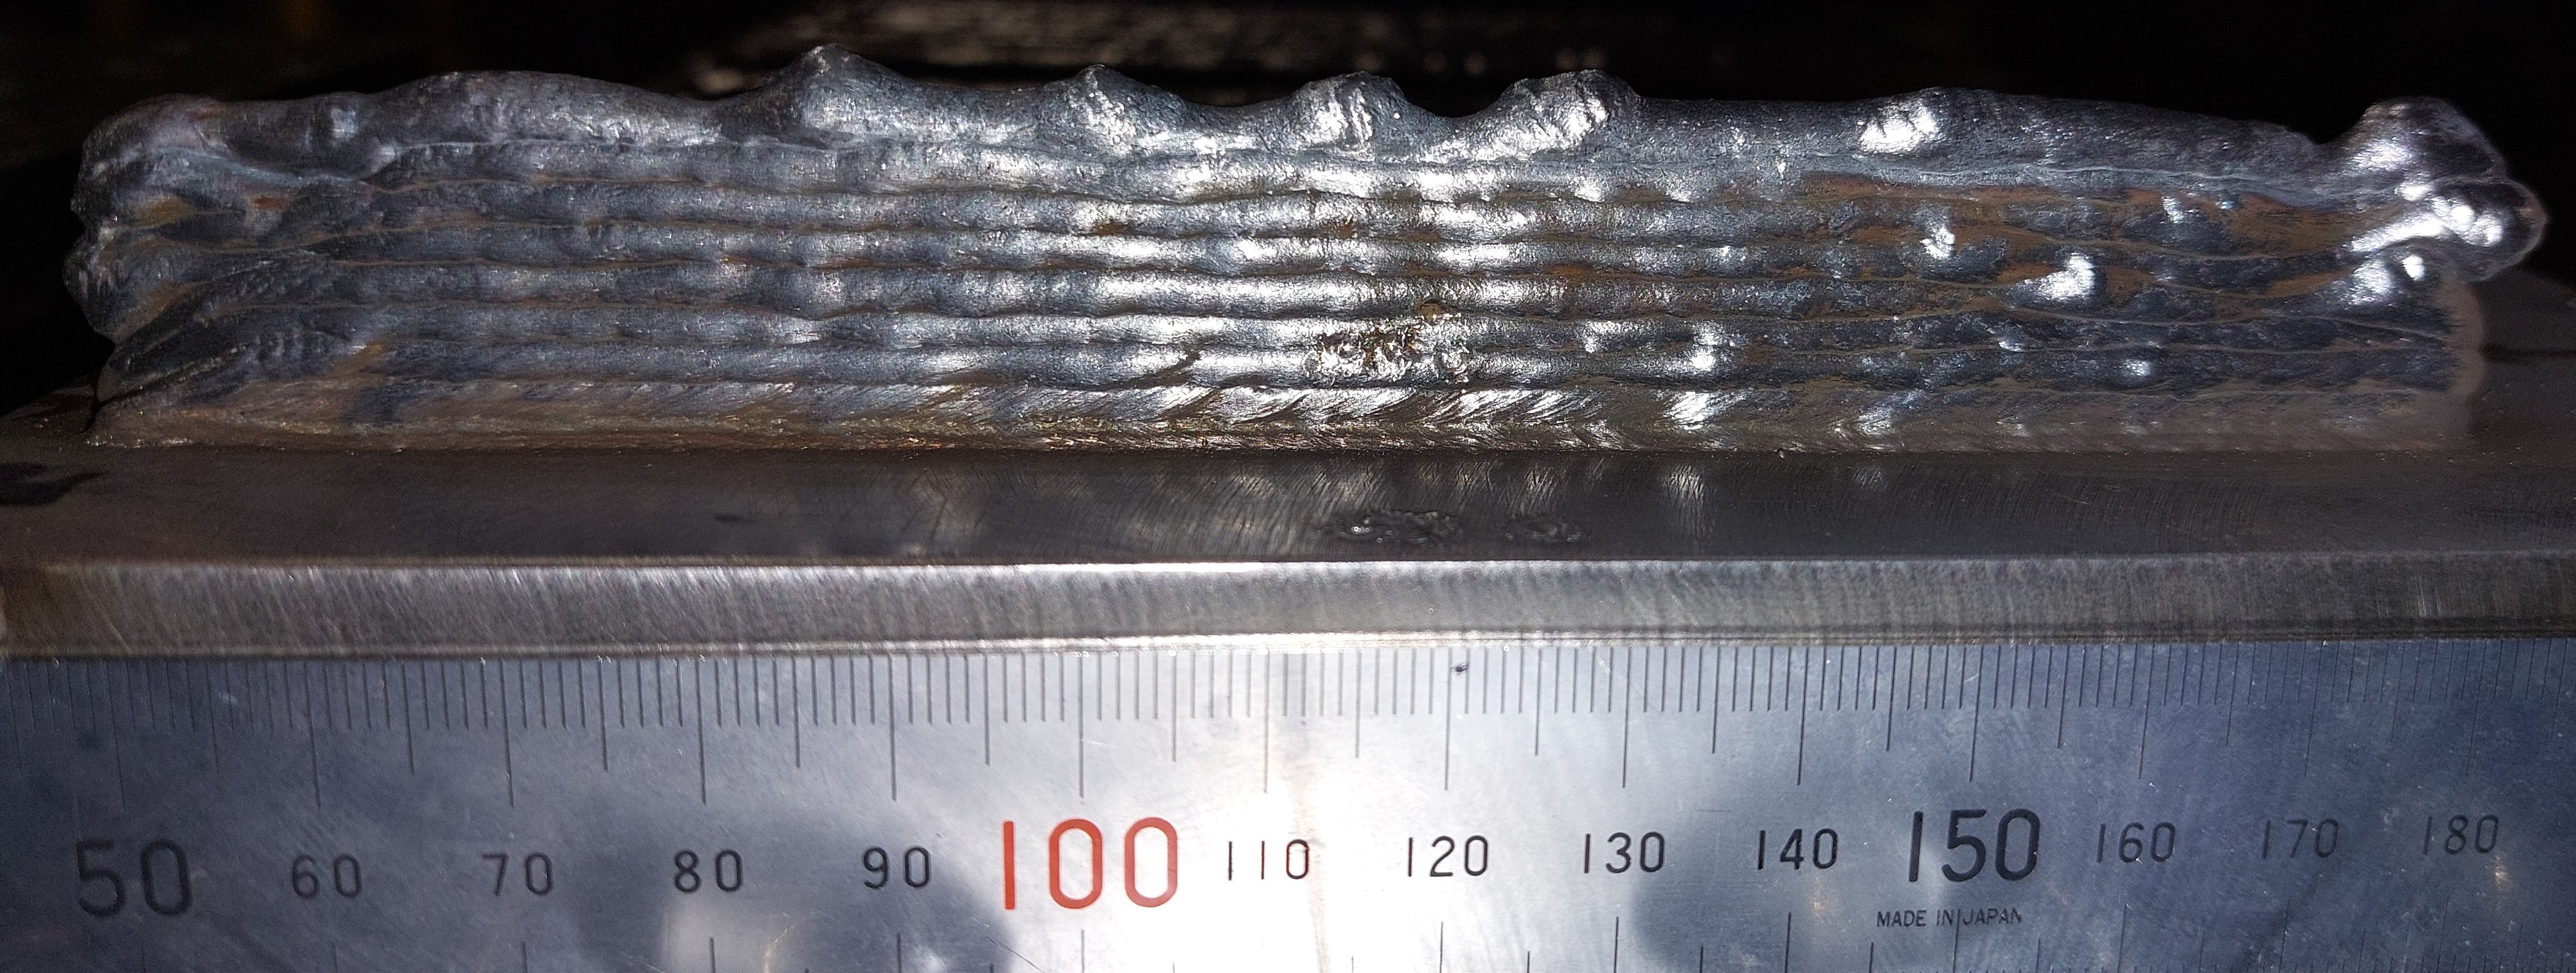
\includegraphics[width=\linewidth]{images/big_wall_1.jpg}
    \captionof{figure}{Final wall test before grinding}
    \label{fig:big_wall_1}
\end{minipage}

This faulty layer was ground to a smooth surface, and an arc length correction of -0.3 was applied, meaning the arc length was reduced by 30\%. This increases the force of the arc on the melt pool by narrowing the arc, and allows for more penetration and re-melting of previous layers to fill in any defects. The resulting wall is shown in \autoref{fig:big_wall_2}, and clearly this change stabilized the process sufficiently to yield relatively smooth layers even after 20 layers.

\begin{minipage}{\linewidth}
    \centering
    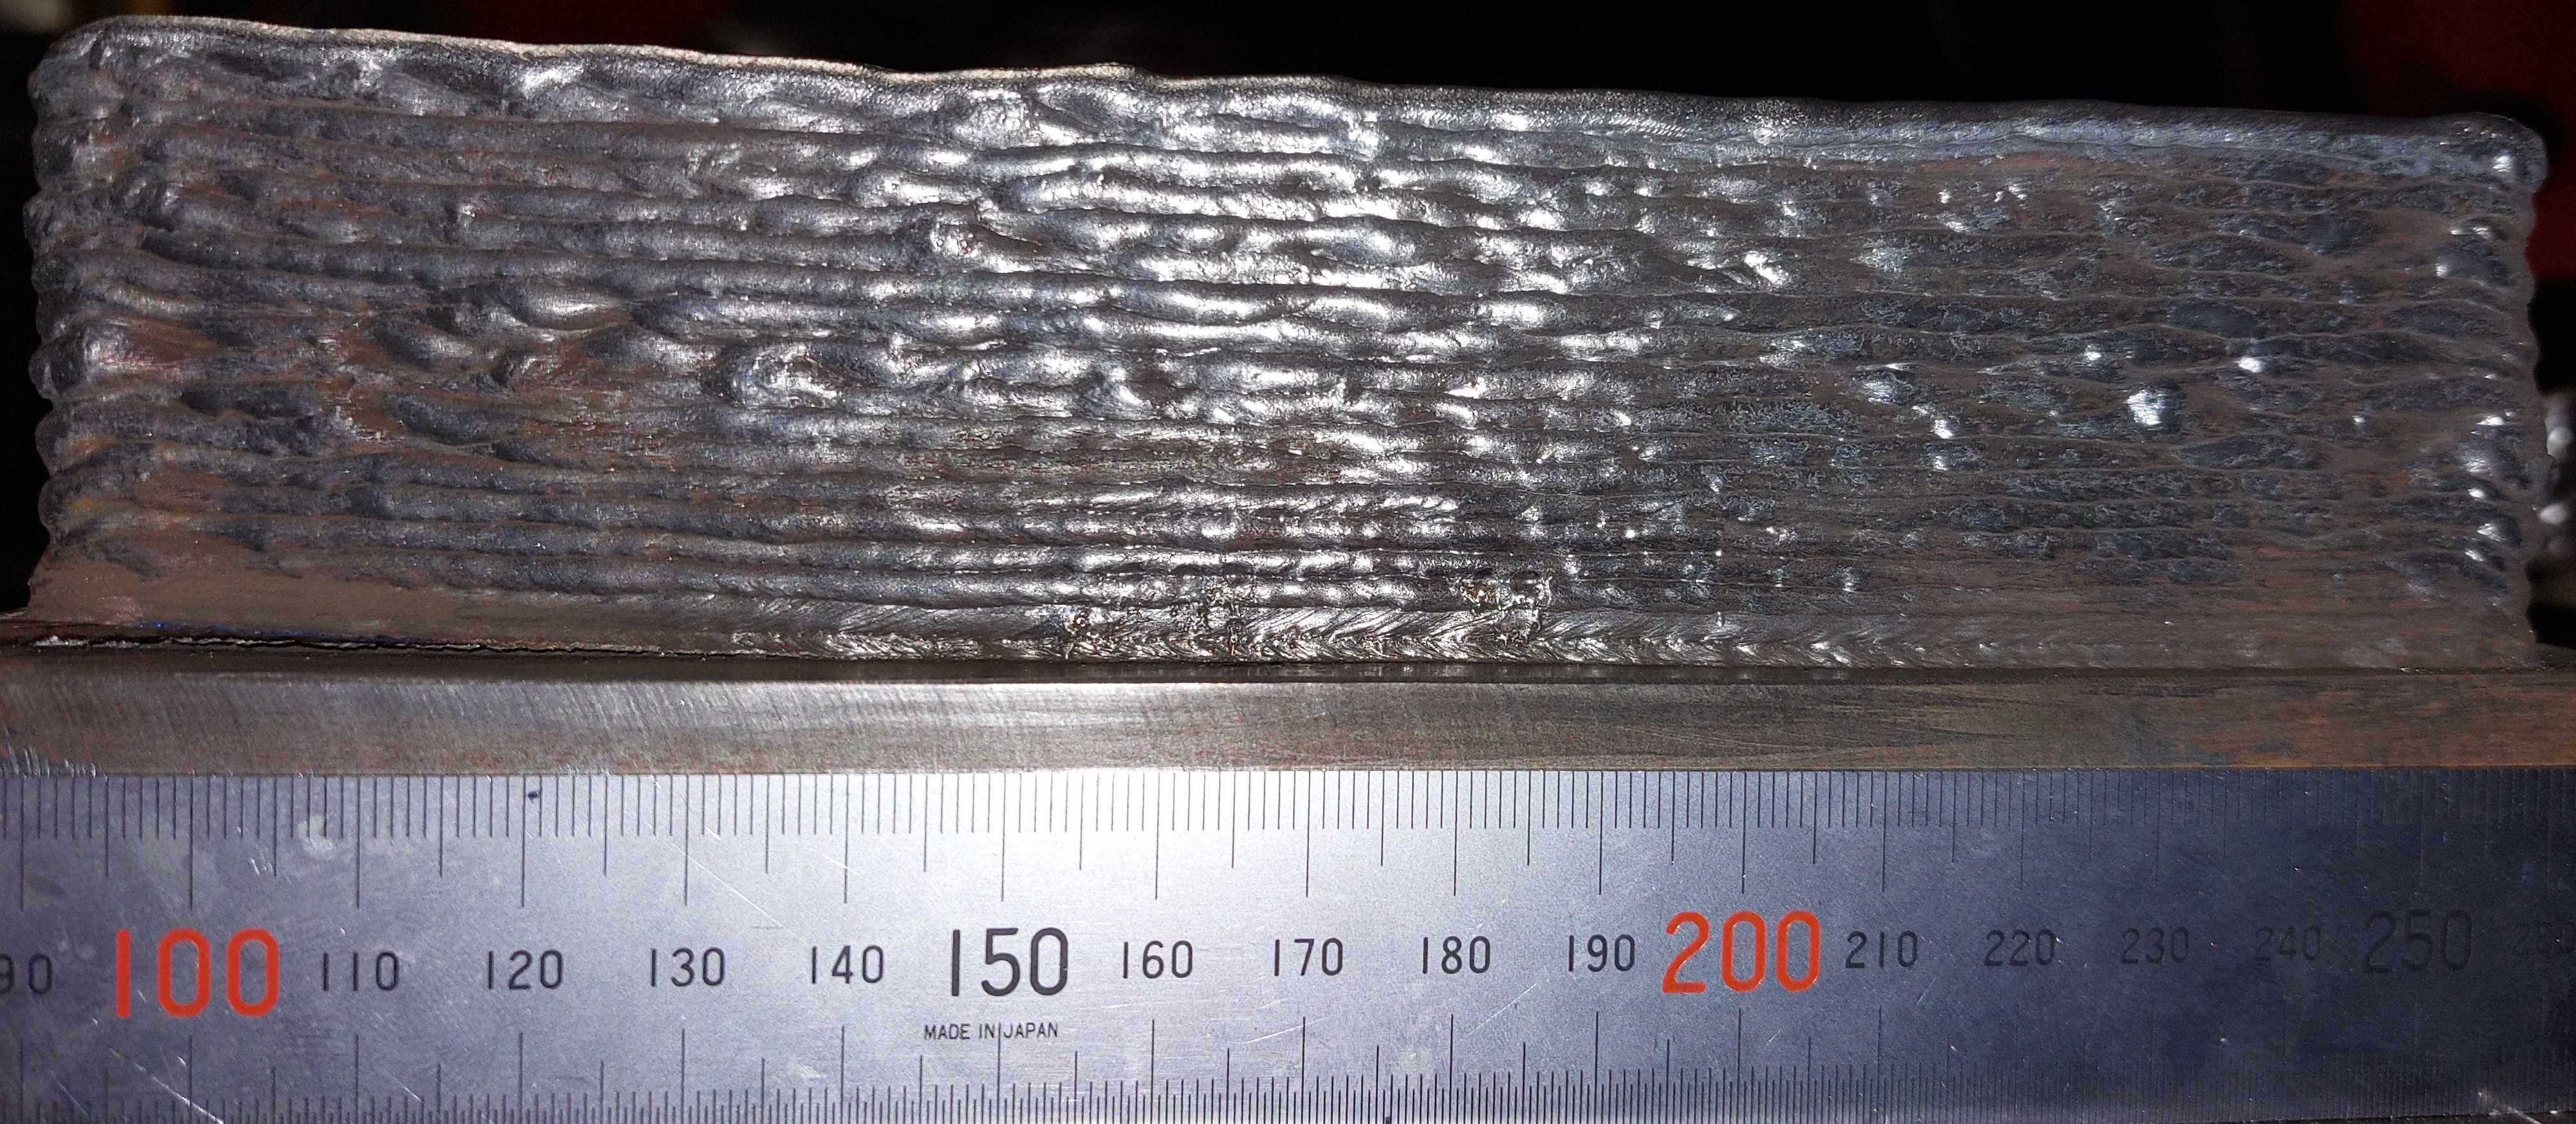
\includegraphics[width=\linewidth]{images/big_wall_2.jpg}
    \captionof{figure}{Final wall test after grinding}
    \label{fig:big_wall_2}
\end{minipage}

Another possible source of inconsistencies was identified after this test: by welding hot, the welding tip can be worn out and its exit hole become larger than desired, as shown in \autoref{fig:tip_hole}. The wire being tested was wound on its spool with residual tension, causing it to come out of the torch at an angle, and this angle can change over time duing welding, deflecting the arc from the intended bead path, causing the same kind of arc and melt pool wandering described earlier.

\begin{minipage}{\linewidth}
    \centering
    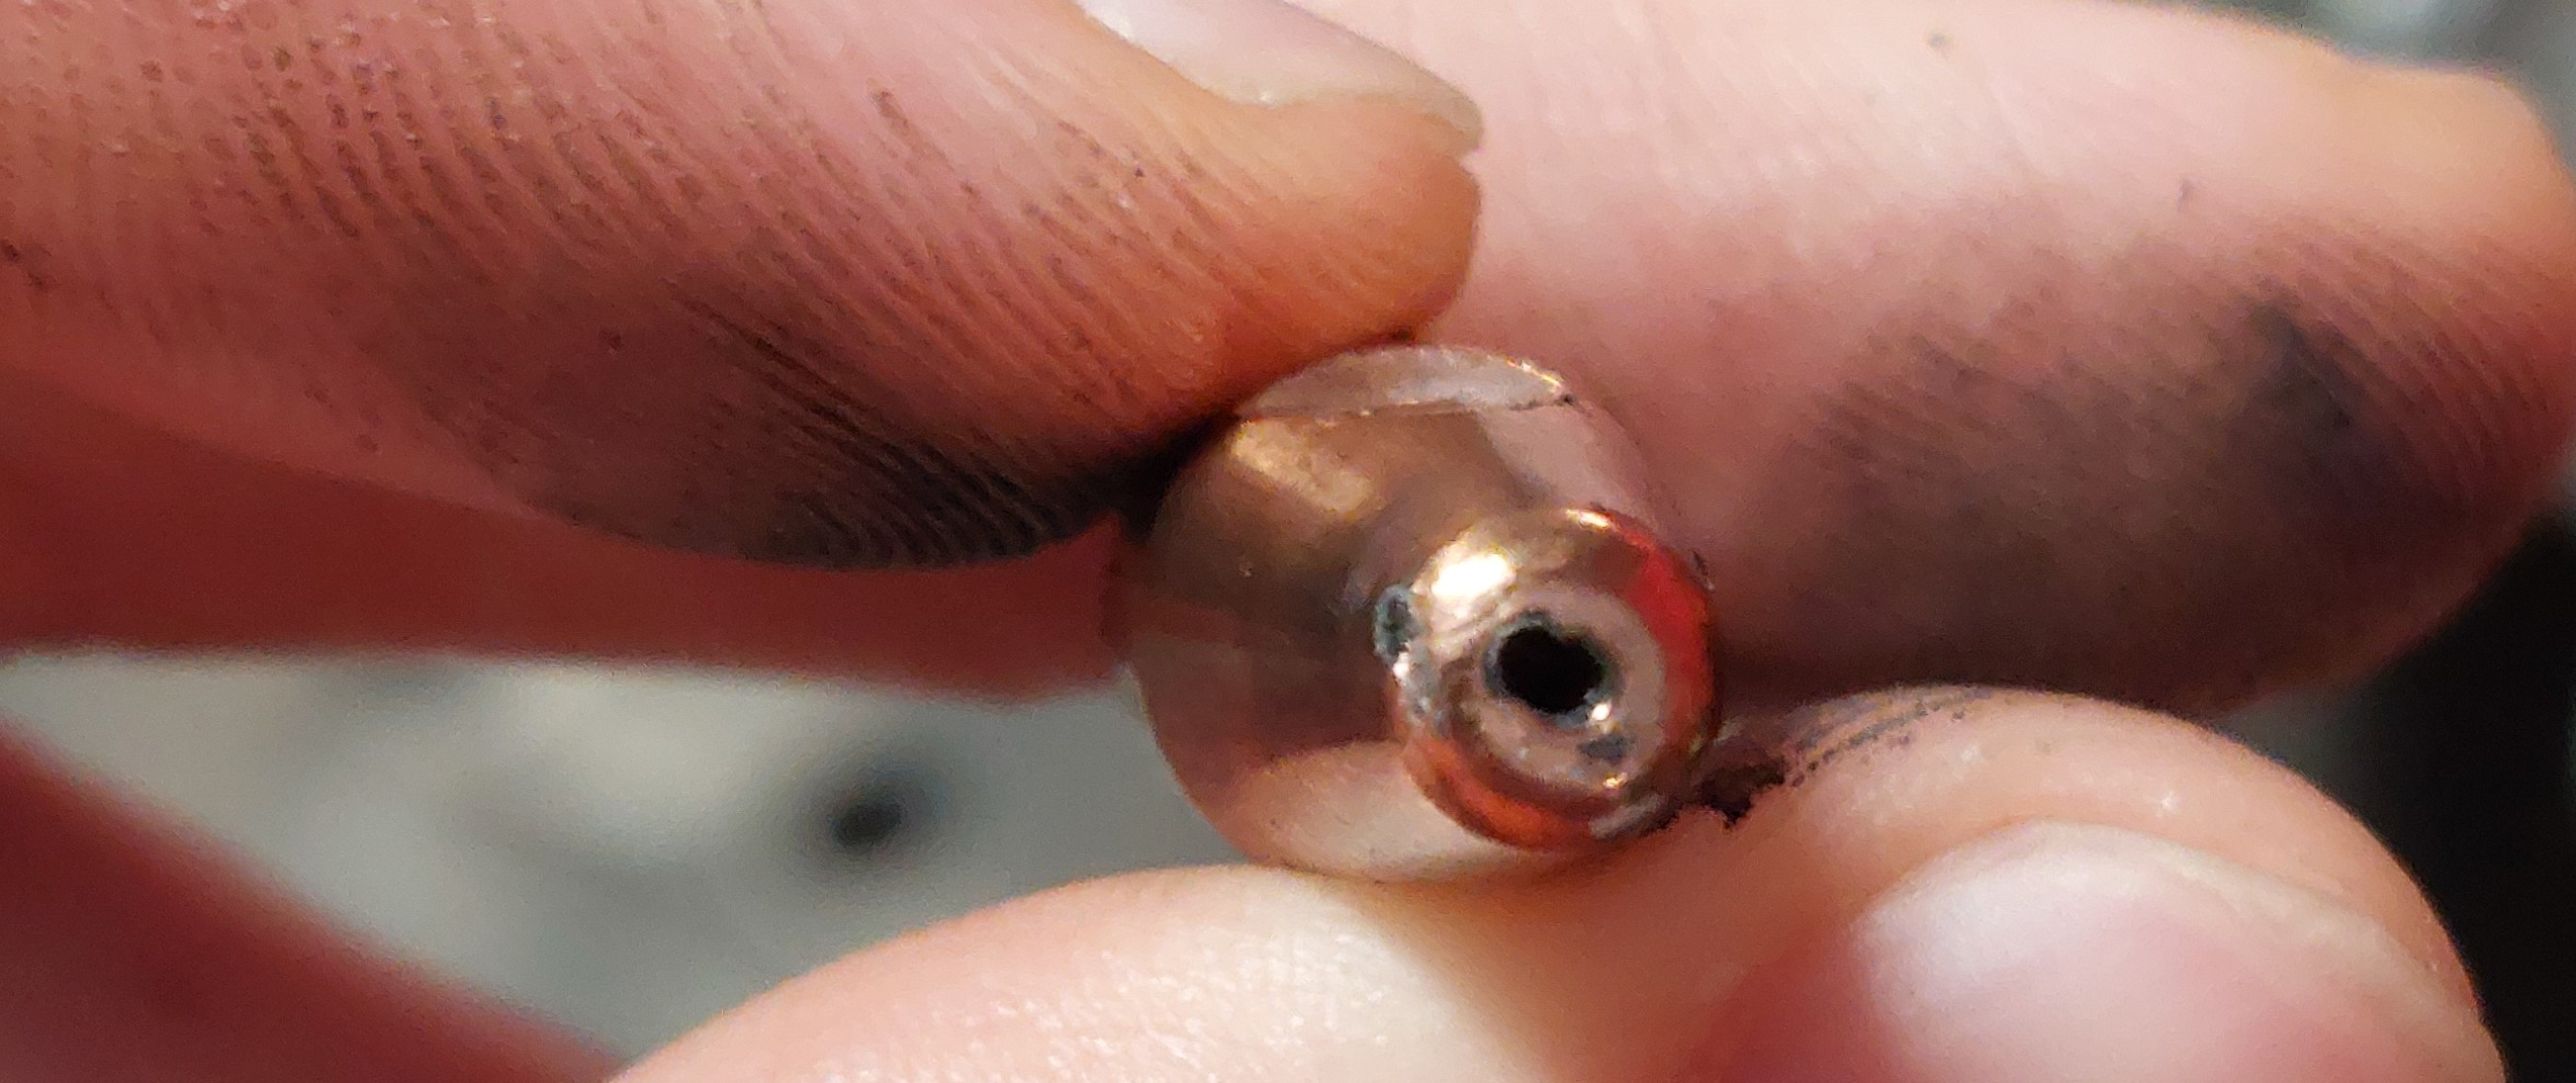
\includegraphics[width=\linewidth]{images/tip_hole.jpg}
    \captionof{figure}{Tip hole wearing out}
    \label{fig:tip_hole}
\end{minipage}

After the establishment of successful single-bead layers, the next milestone was the minimum print quality for a full-scale part. The chosen geometry was a simple set of concentric rings, and the initial tests were conducted on a single ring.
This involved manually rotating the layer toolpaths around the center axis to randomize the start/stop points of the beads to prevent defects from accumulating in the same place, as well as alternating the direction of welding. The resulting ring is shown in \autoref{fig:ring_1}.

\begin{minipage}{\linewidth}
    \centering
    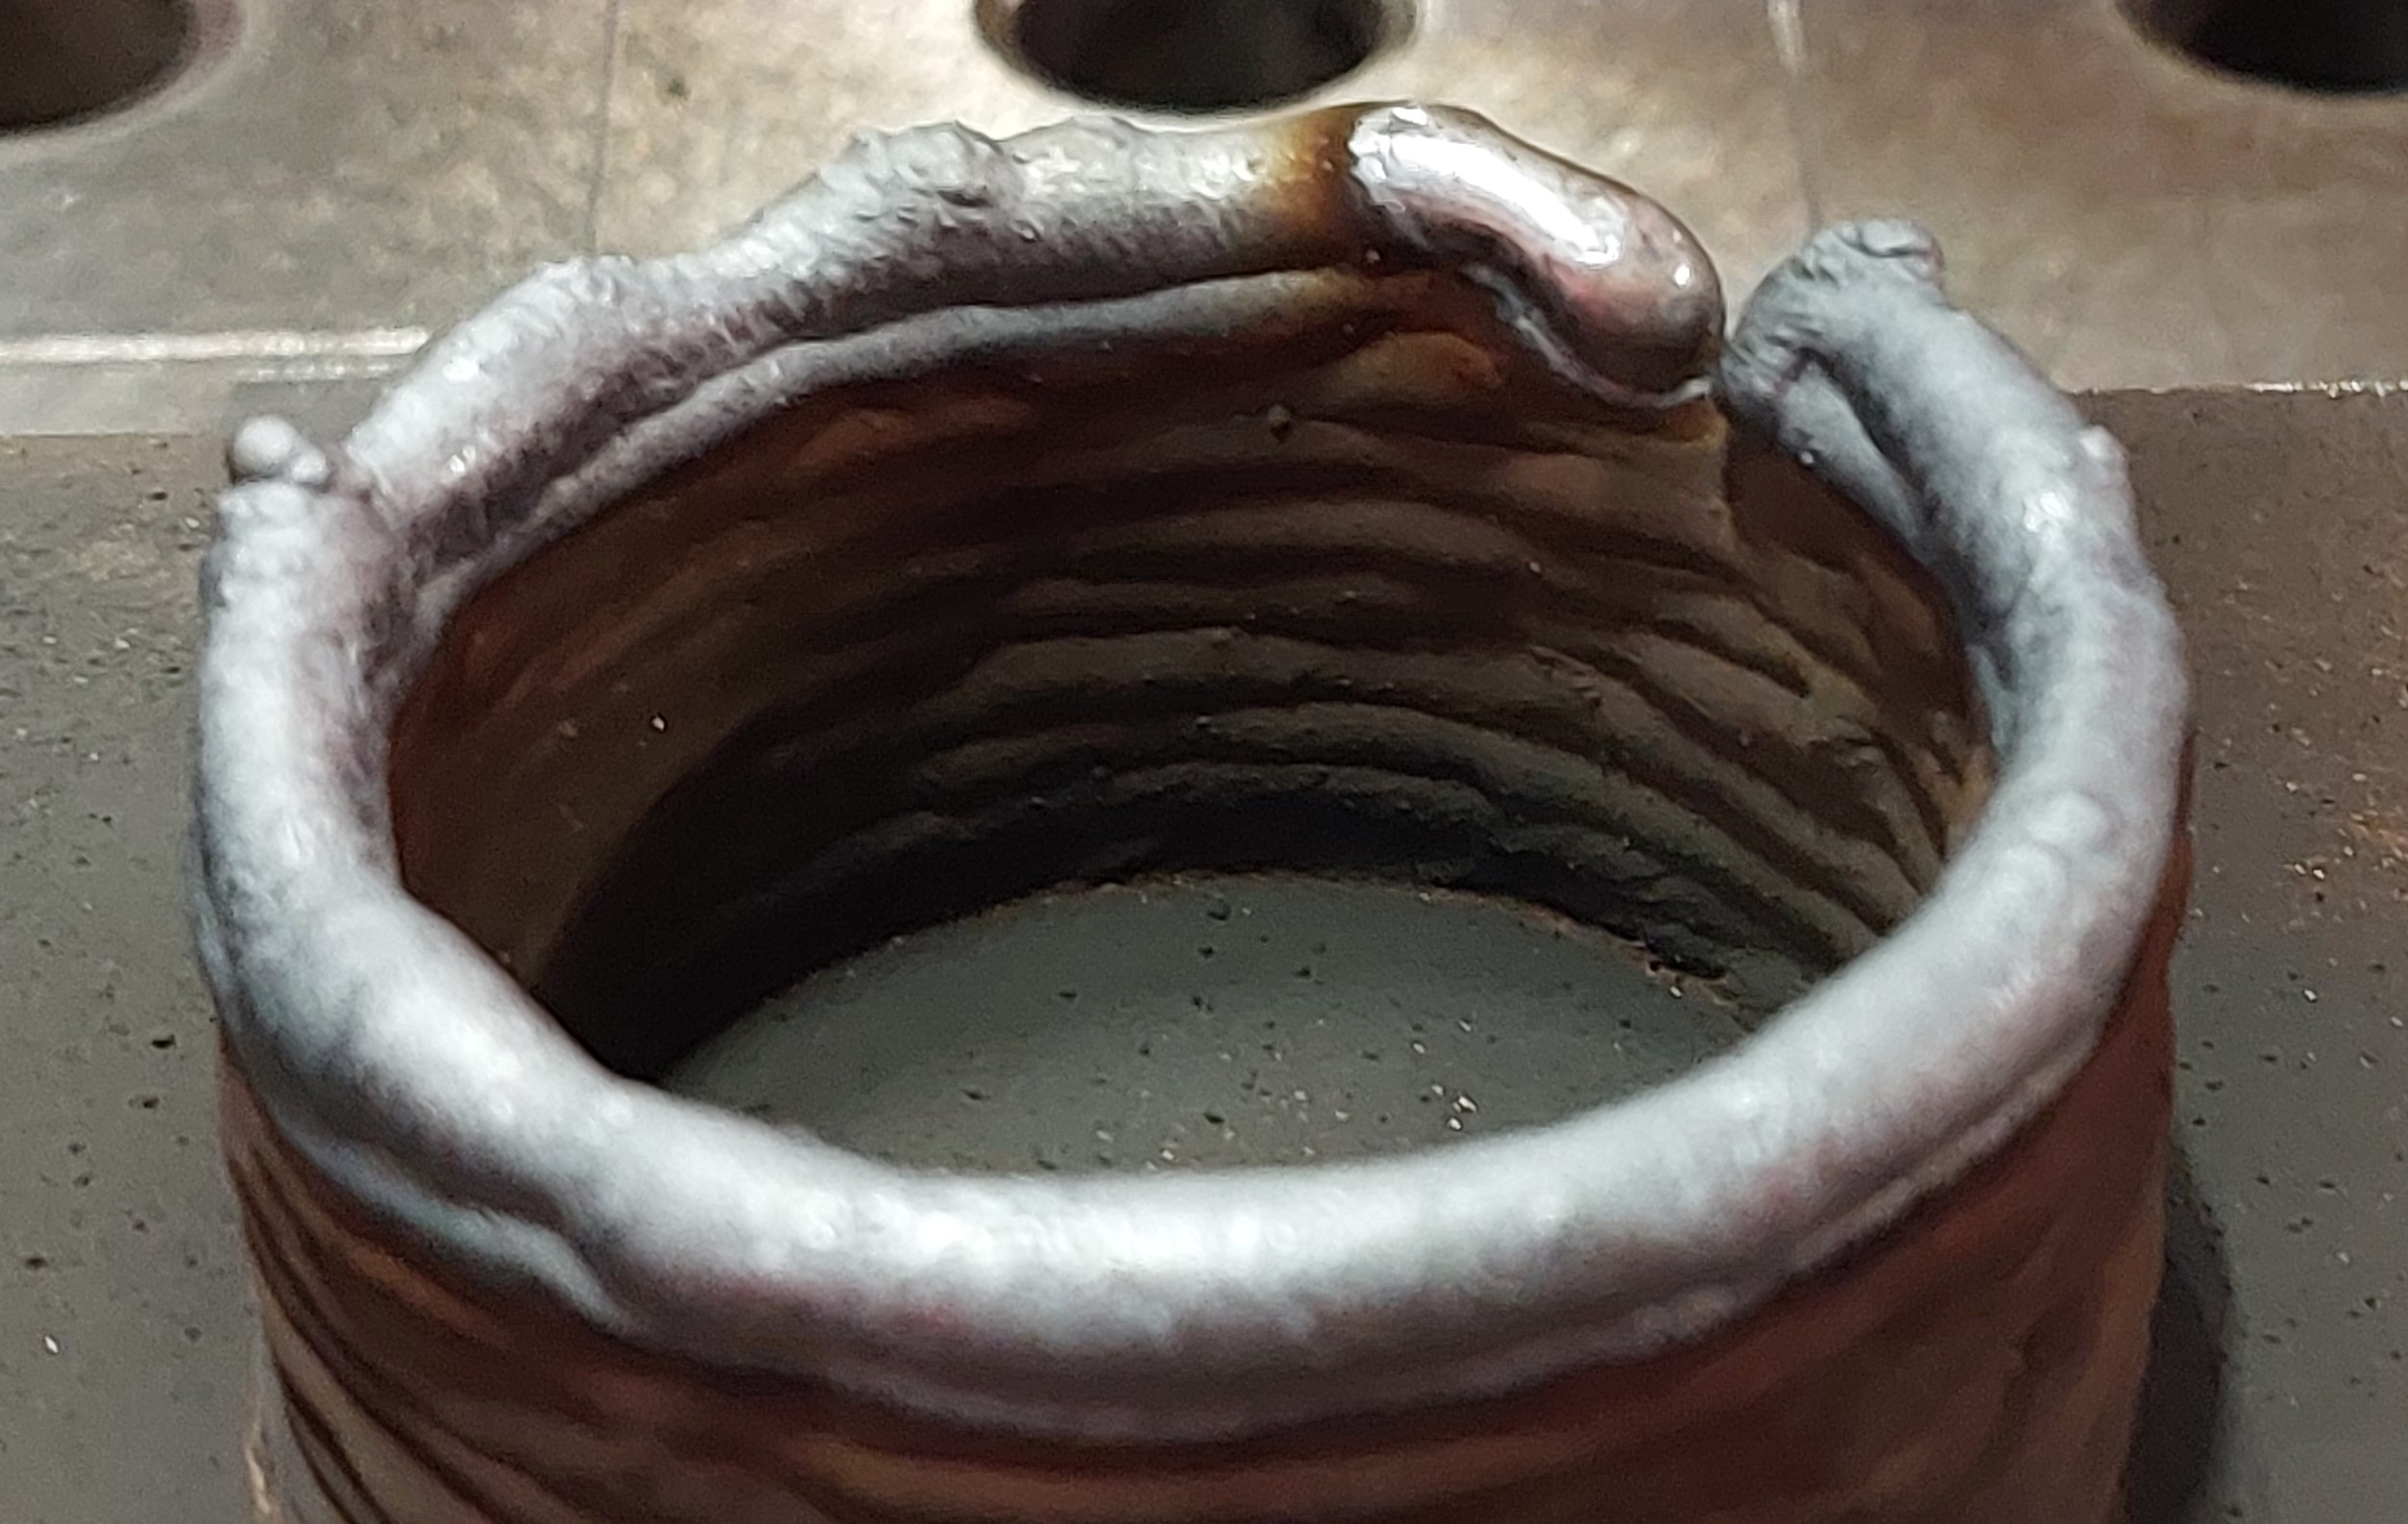
\includegraphics[width=\linewidth]{images/ring_1.jpg}
    \captionof{figure}{First ring test with defect}
    \label{fig:ring_1}
\end{minipage}

The rather large defect was caused by a previous layer containing a large valley, and the arc being unable to close it, as shown in \autoref{fig:ring_defect}.

\begin{minipage}{\linewidth}
    \centering
    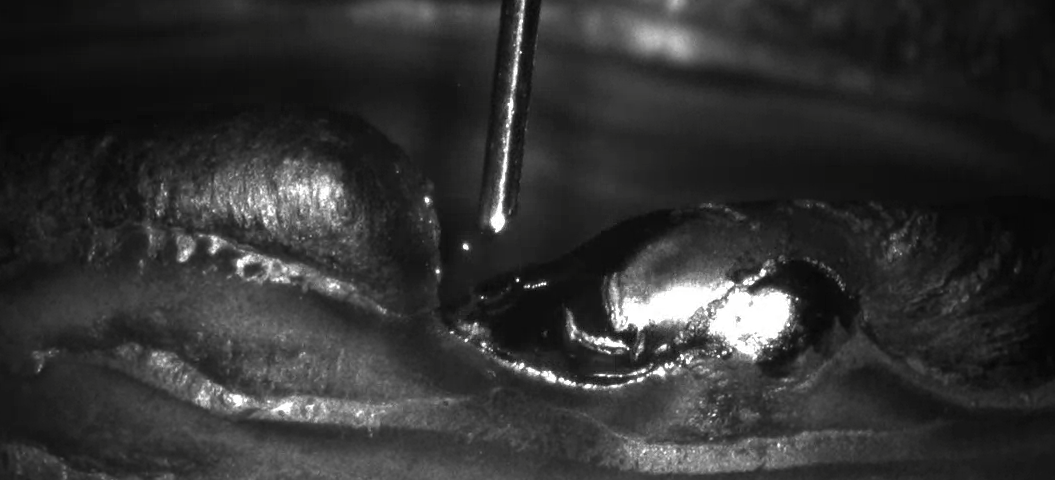
\includegraphics[width=\linewidth]{images/ring_defect.PNG}
    \captionof{figure}{Moment of inability to close gap in first ring test}
    \label{fig:ring_defect}
\end{minipage}

Welding was filmed using the previously mentioned Cavitar camera, and analysing the solidification of the melt pool in real-time showed that the source of the defects was not thermal, but rather possibly due to the effects of the oxygen in the atmosphere pulling the elements in the melt pool outwards, causing "bubbling" outgrowths as shown in \autoref{fig:bubble_defect}.

\begin{minipage}{\linewidth}
    \centering
    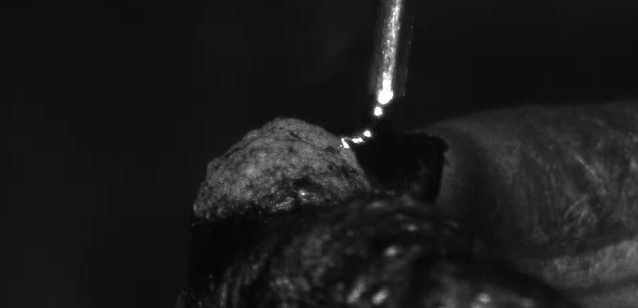
\includegraphics[width=\linewidth]{images/bubble_defect.PNG}
    \captionof{figure}{Bubble outgrowths during welding}
    \label{fig:bubble_defect}
\end{minipage}

This effect would be pronounced in higher layers due to less of the base plate impeding the shielding gas' flow and keeping it in contact with the melt pool for longer, which might have explained why defects consistently ocurred once a certain wall height was reached.

In order to prolong the contact time of the shielding gas with the weld pool, the travel speed was reduced from 0.3 to 0.25 m/min. The interpass temperature was also increased from 50$\deg$ to 80$\deg$ to reduce cooling times and increase the likelihood of layer remelting. A second ring was printed with these conditions, as shown in \autoref{fig:ring_2}.
This ring was the first wall to be printed without any significant defects occurring - most likely due to the mitigation of the oxygen effects by the slower travel speed, and the increased heat input allowing for more re-melting of previous layers to fill in any defects. This second point is important, since defects cannot be prevented, but they can be corrected through remelting.

\begin{minipage}{\linewidth}
    \centering
    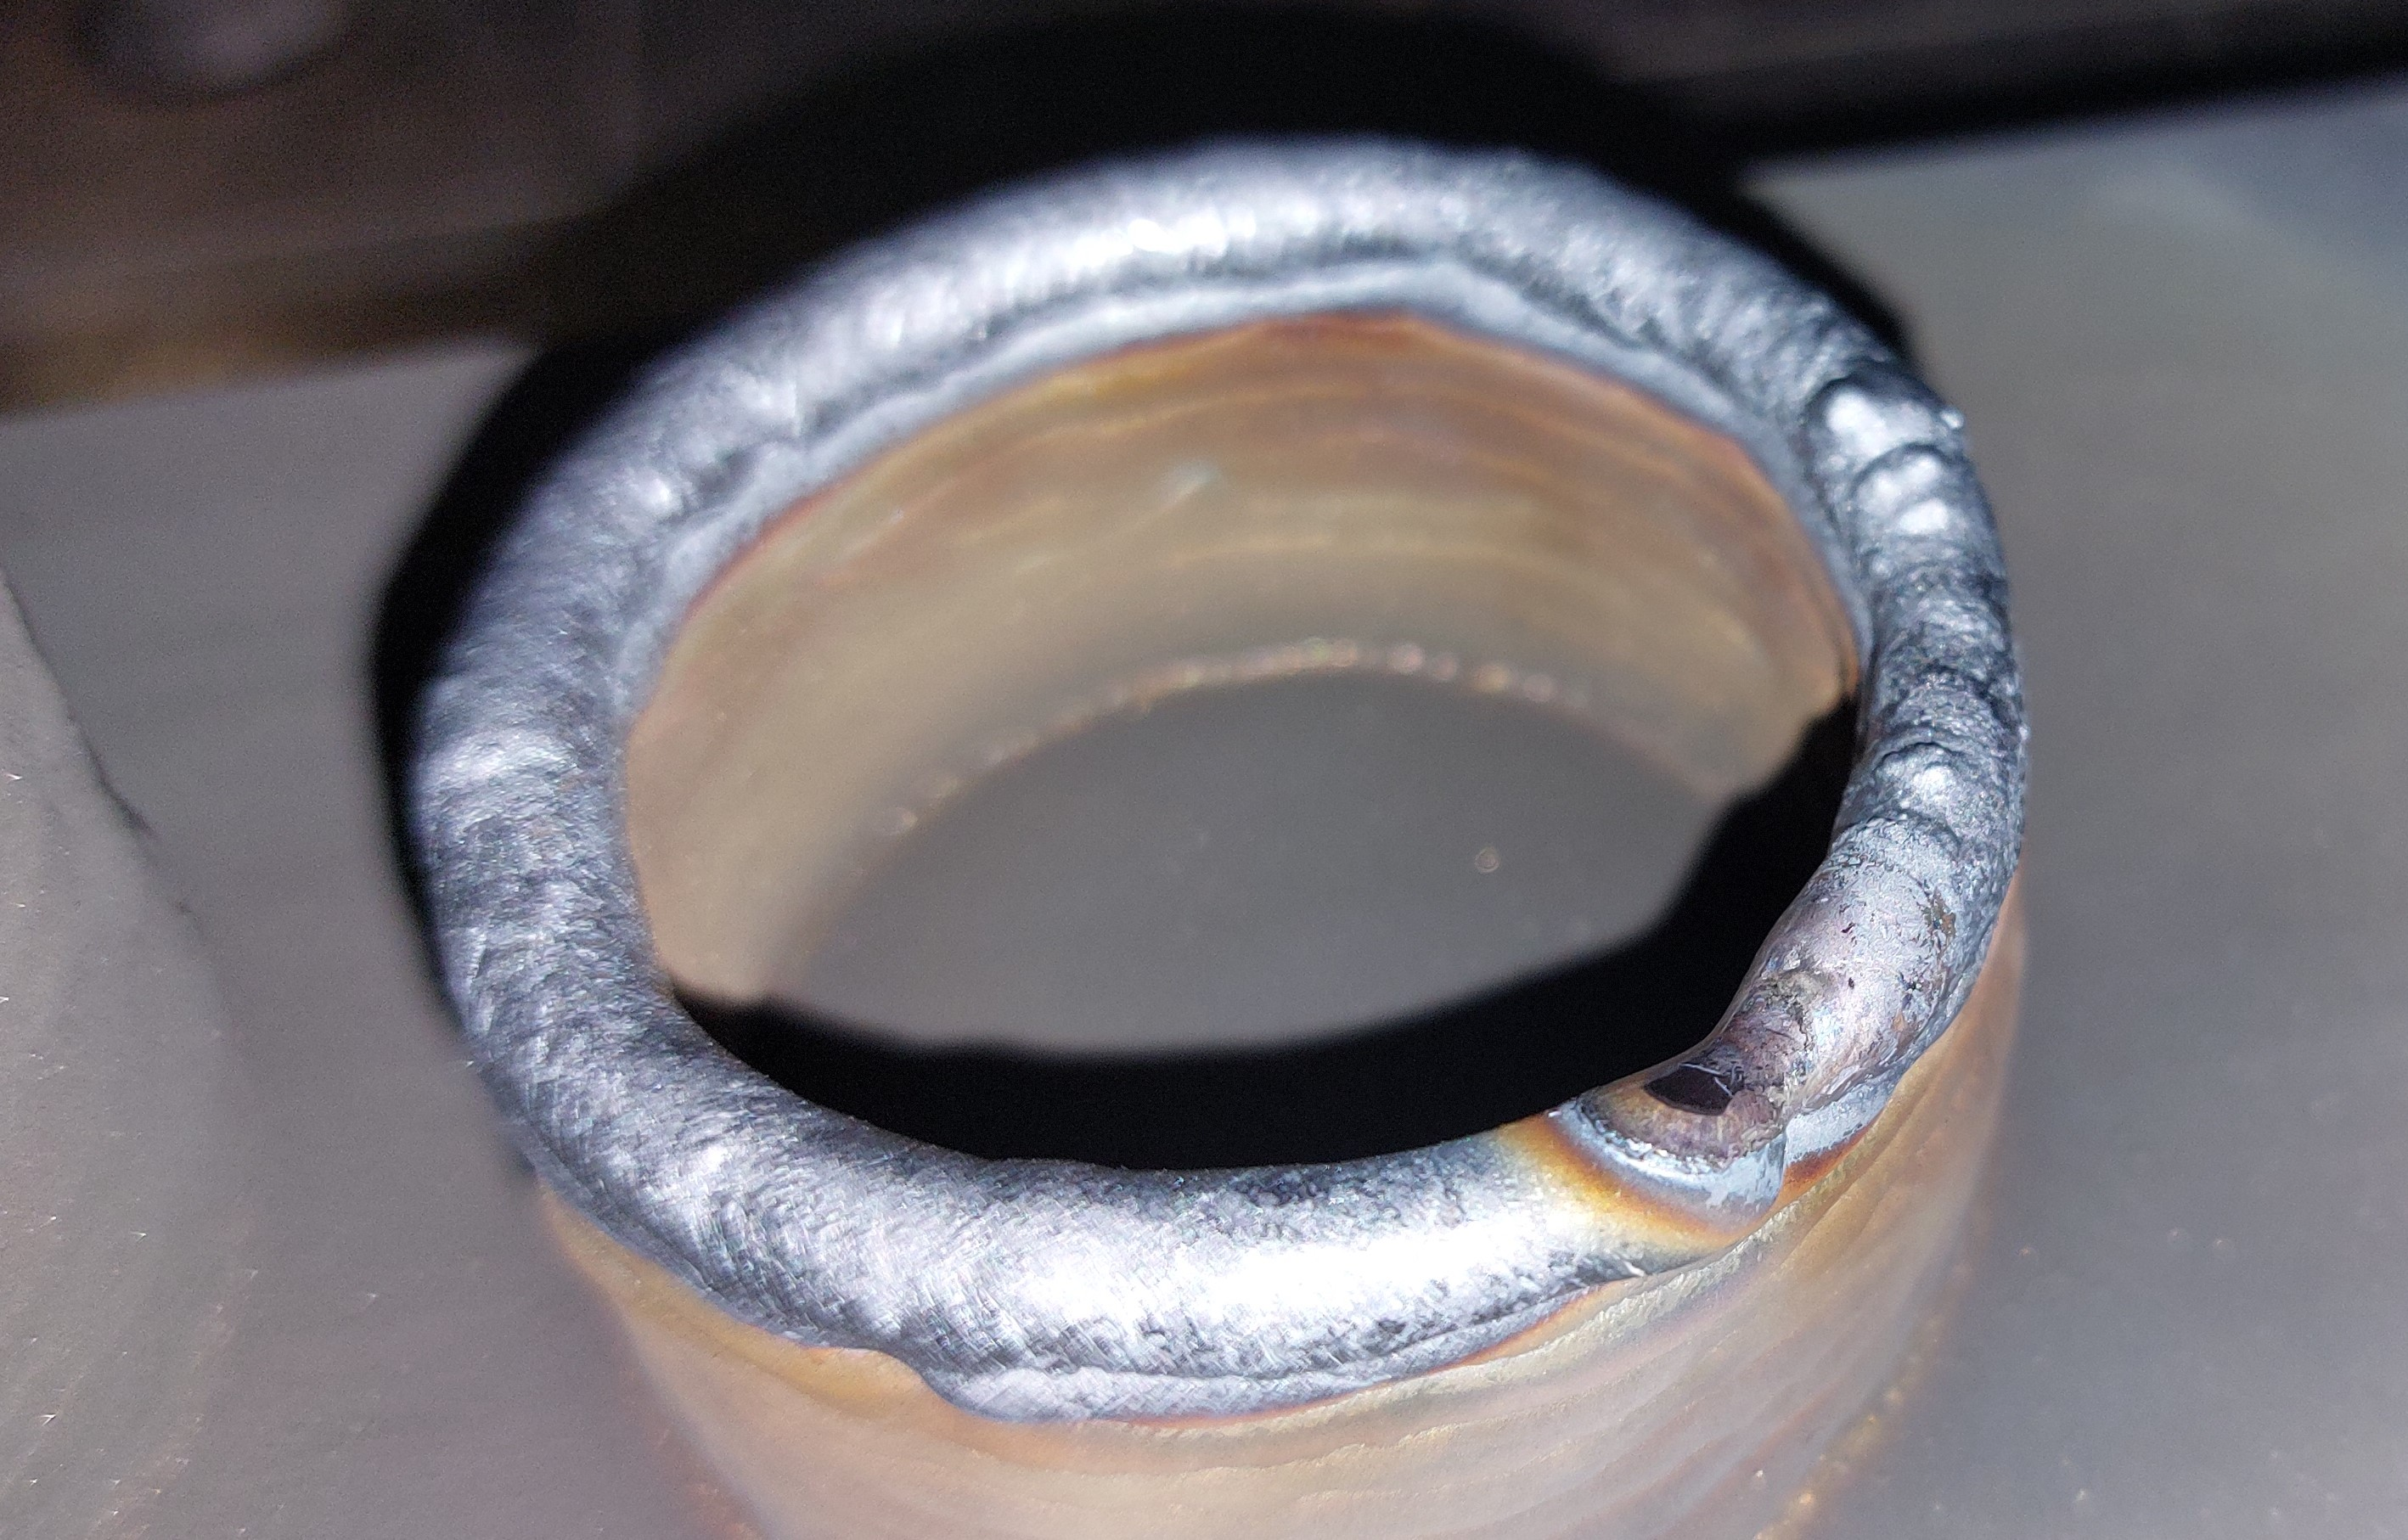
\includegraphics[width=\linewidth]{images/ring_2.jpg}
    \captionof{figure}{Second ring test with no defects}
    \label{fig:ring_2}
\end{minipage}

With this relatively stable condition achieved, this ring was used for sample collection for microscopy and magnetic testing. The tests moved on to printing full geometries consisting of two concentric rings on much smaller baseplates, which are commonly used in production scenarios. This introduced a new issue of thermal loading and excessively long cooling times due to the comparatively small thermal reservoir a smaller baseplate offers.

\begin{minipage}{\linewidth}
    \centering
    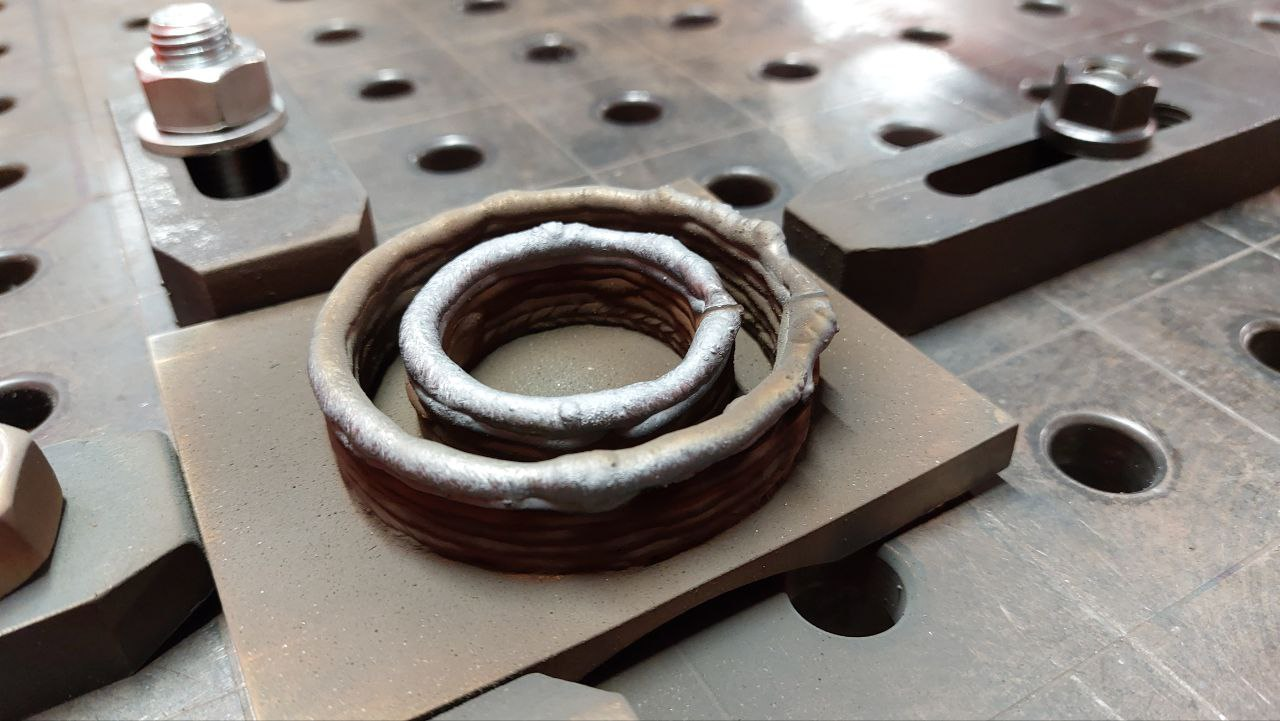
\includegraphics[width=\linewidth]{images/photo_2023-11-14_15-40-54.jpg}
    \captionof{figure}{First full geometry print in progress}
    \label{fig:half_ring_bending}
\end{minipage}

As shown in \autoref{fig:half_ring_bending}, the corners of the small baseplate are lifted due to repeated heating, and we begin to see the development of so-called "humps" after a few layers. The first few layers in this print were fully smooth and stable. We considered that the bending of the plate may have introduced wire tip positioning errors and thus induced instabilities, so the MaxQ geometrical scanning system was configured for the next print. This system projects the planned toolpath on the existing geometry and adjusts the vertical distance to the part accordingly to keep a stable Contact Tube to Work Piece (CTWD) distance. All subsequent prints made use of this distance correction through 3D scanning. 

\begin{minipage}{\linewidth}
    \centering
    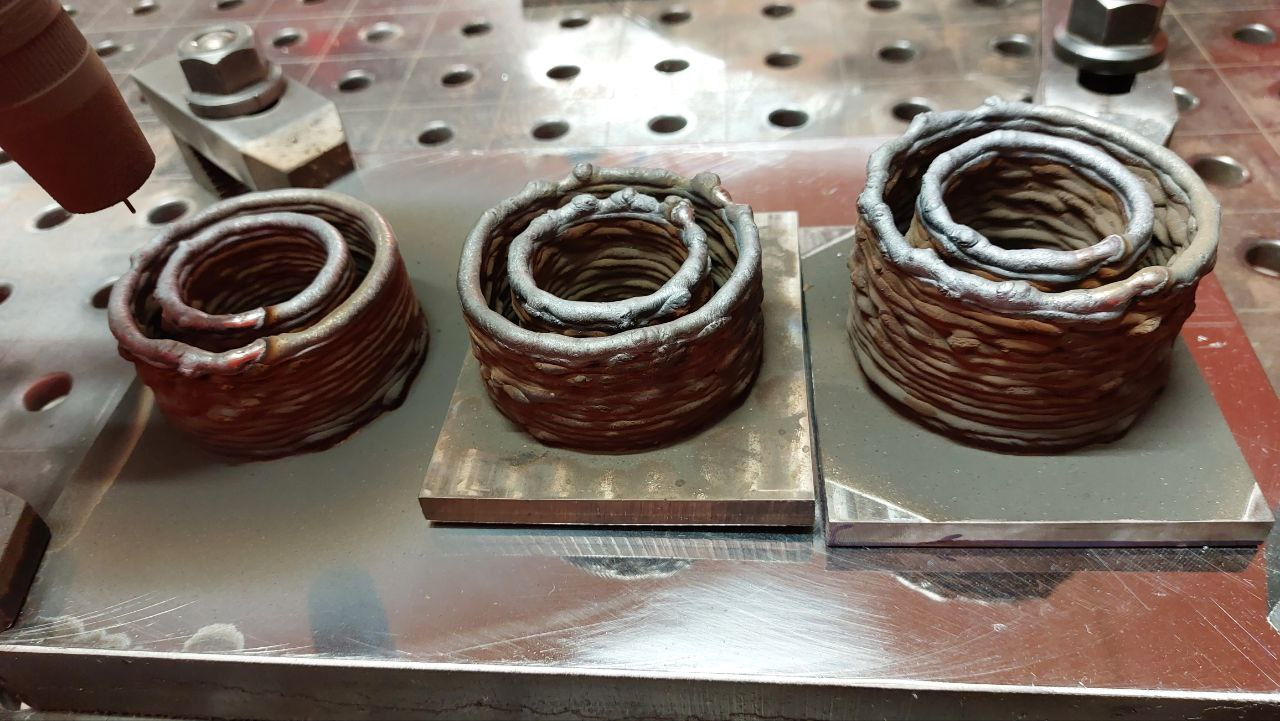
\includegraphics[width=\linewidth]{images/photo_2023-11-14_15-39-49.jpg}
    \captionof{figure}{Three full geometry attempts}
    \label{fig:3_rings}
\end{minipage}

\autoref{fig:3_rings} shows three subsequent tests at printing the full geometry in varying conditions. In the center is the finished piece previously shown in \autoref{fig:half_ring_bending}, which was printed with an interpass temperature of 80 $^o$C, displaying significant defects on its top layer. On the right, the following print can be seen. The shielding gas flow rate, which was previously 22 L/m, was increased to 24 L/m. Because of the baseplate's composition (also Vacoflux 17), wettability issues had been identified elsewhere and mitigated with a heat input increase of 15\%, 10\% and 5\% for the first three layers. This was also done for this print. 3D scanning was used along with clamps on the edges of the baseplate to address bending and thus mitigate positioning issues. The interpass temperature was also set to 120 $^o$C to reduce cooling times, but still with all of these process changes, defects still occurred to a significant degree. The hypothesis arose that this may be due to the melt pool staying hot for too long (due to poor thermal conduction of the thin walls of the part), and being exposed to the atmosphere while still in a liquid state, causing reactions with the oxygen present.

As pictured on the very left, another test was run on a large baseplate. This was done to examine whether the thermal issues were the true cause behind the "hump" defects. The interpass temperature was lowered to 50 $^o$C, and additionally, a leading angle of 10 degrees (i.e. the tip tilted in the direction of travel) was introduced in order to push the melt pool forwards, remelting defective layers, instead of backwards, where the forces might accumulate to further defects. Even with these process parameter changes, the defects continued to occur, although quite often, it was possible to remelt previously defective layers.

It must be said that for all of these "humping" and (as mentioned above) "bubbling" defects, the location of the errors was seemingly random and did not follow any discernible patterns. Previous defects were more often than not successfully corrected by a new layer, which in turn had new defects in a different part of the ring.

% \subsection{Software defects}

% ROS bridge
% Decryption of the Techman
% Post-processor minor errors
% Techman weirdness (not starting, bugging out)
% TCP errors
% MaxQ 3D camera calibration issues

\begin{table*}[ht]
\centering
\caption{VSM Hysteresis Loop Results}
\label{tab:mag_data}
\begin{tabular}{|l|l|l|l|l|l|}
\hline
\textbf{Property/Sample} & \textbf{Wire} & \textbf{Weld} & \textbf{Ar} & \textbf{H} & \textbf{H \%} \\ \hline
\textbf{Coercivity [A/m]}         & 530.78   & 659  & 934  & 362  & -31.87 \\ \hline
\textbf{Remanence [A/m]}          & 34.94    & 32.2 & 25.4 & 18.3 & -47.56 \\ \hline
\textbf{Sat. Magnetization [A/m]} & 1906.847 & 1883 & 1832 & 1821 & -4.46  \\ \hline
\textbf{Max. Permeability [H/m]}  & 5240.246 & 3810 & 3002 & 4009 & -23.49 \\ \hline
\textbf{Hysteresis Area [J/m$^3$]}  & 36.377   & 39.9 & 34.8 & 26.5 & -27.28 \\ \hline
\end{tabular}
\end{table*}

